\documentclass{article}


\usepackage[T2A]{fontenc}
\usepackage[utf8]{inputenc}
\usepackage[russian]{babel}
\usepackage{float}

\usepackage[unicode, colorlinks, linkcolor=blue]{hyperref}

\usepackage{graphicx}
\graphicspath{{pictures/}}
\DeclareGraphicsExtensions{.pdf,.png,.jpg}


\begin{document}
%----------------------------------Шапка---------------------------------------------
	\begin{center}
		
\includegraphics[scale=0.25]{AU}\\
		{\Large\bfseries Санкт-Петербургский национальный исследовательский Академический университет имени Ж.И.~Алфёрова Российской академии наук}
	\end{center}

	\begin{center}
		Свиридов Фёдор, Александр Слободнюк, Владимир Попов
	\end{center}
	\rule{12cm}{0.4mm}
	\begin{center}
		{\large\textbf{Рабочий протокол и отчёт по лабораторной работе № 4}}
	\end{center}
%--------------------------------------------------------------------------------------
\paragraph{Цель работы.}
С помощью баллистического маятника определить скорости пуль с различными массами

\paragraph{Задачи, решаемые при выполнении работы.}
\begin{itemize}
	\item Измерить массы пуль
	\item Измерить длину баллистического маятника
	\item Измерить массу баллистического маятника
	\item Измерить отклонения маятника после выстрела каждой пули
	\item Обработать полученные результаты
	\item Сделать выводы
\end{itemize}

\paragraph{Объект исследования.}
Зависимость скорости пули от её массы после выстрела из пружинного пистолета

\paragraph{Метод экспериментального исследования.}
Измерение скоростей пуль

 \paragraph{Рабочие формулы и исходные данные.}\hypertarget{formuls}{}
 \begin{flushleft}
 	Предполагаемая зависимость скорости пули от её массы после выстрела из пружинного пистолета: $ v\sim\sqrt{\frac{1}{m}}$
 \end{flushleft}

\begin{equation}
	\fbox{$v_i=\frac{m_i+M}{m_i}\sqrt{\frac{g}{l}}\cdot x_i$}
\end{equation}
 	где $l$ - длина маятника; $m_i$ и $x_i$ - масса пули и отклонение маятника в данном эксперименте, соответственно

\begin{table}[h]
	\caption{\bf Измерительные приборы}
	\begin{tabular}[c]{|p{7.5em}|p{7.5em}|p{7.5em}| p{7.5em}|}
		\hline
		Наименование & Тип прибора & Используемый диапазон & Погрешность прибора\\\hline
		Линейка & Аналоговый & $20 - 40\quad\mbox{см}$ & 0,1 см\\
		\hline
		Электронные весы& Цифровой & $1 - 200\quad\mbox{г}$ & 0,01 г \\
		\hline
	\end{tabular}
\end{table}

 \begin{figure}[htb]
 	\caption{Схема установки}
\centering 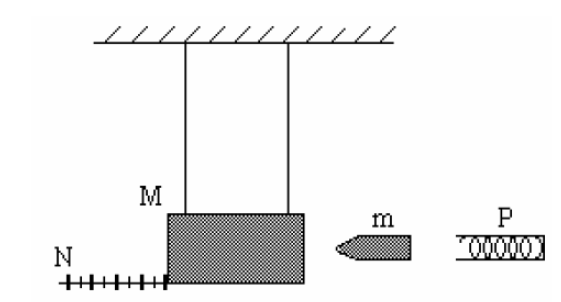
\includegraphics[scale=0.5]{схема}
 \end{figure}

\paragraph{Результаты прямых измерений и их обработки}
\begin{itemize}
	\item Масса баллистического маятника: $ M=112\;\mbox{г} $ 
	\item Длина маятника: $ l=30\;\mbox{см}$
\end{itemize}
		
		\begin{table}[htb]
			\centering
		\caption{Измерения}
		\begin{tabular}{| c | c | c |}
			\hline
			№ & Масса пули (г) & Отклонение маятника (см) \\
			\hline
			1 & 11,53 & 9 \\
			\hline
			2 & 10,72 & 5 \\
			\hline
			3 & 3,74 & 2,5 \\
			\hline
		\end{tabular}
	\end{table}

\paragraph{Расчет результатов косвенных измерений}
Пользуясь \hyperlink{formuls}{формулой (1)}, находим скорости пуль:
\begin{table}[!htb]
	\centering
	
	\begin{tabular}{|c|c|}
		\hline
		№ & Скорость пули ($\frac{\mbox{м}}{\mbox{с}}$) \\
		\hline
		1 &  5,51  \\
		\hline
		2 &  3,27  \\
		\hline
		3 & 4,42  \\
		\hline
	\end{tabular}
\end{table}



\end{document}
